% The Lynette Gate -- effects on VeriContest ProofGen scoring
% UIUC SRSE 2026, August 25, 2026
% Build: pdflatex lynette-gate.tex  (run twice)

\documentclass[aspectratio=169,10pt]{beamer}

\usepackage[T1]{fontenc}
\usepackage[utf8]{inputenc}
\usepackage[sfdefault]{FiraSans}
\usepackage[scaled=0.85]{FiraMono}
\usepackage{listings}
\usepackage{tikz}
\usepackage{tcolorbox}
\usepackage{booktabs}

\usetheme{metropolis}
\metroset{sectionpage=none, numbering=fraction, progressbar=frametitle}

\usetikzlibrary{arrows.meta, positioning, calc, fit, backgrounds}
\tcbuselibrary{skins}

% Palette
\definecolor{lgInk}{HTML}{23373B}
\definecolor{lgAccent}{HTML}{C25E00}
\definecolor{lgTeal}{HTML}{0F7B8A}
\definecolor{lgRed}{HTML}{B3282D}
\definecolor{lgGreen}{HTML}{2E7D32}
\definecolor{lgGrey}{HTML}{6B7A7D}
\definecolor{lgWash}{HTML}{F2F4F4}
\definecolor{lgWashWarm}{HTML}{FBF1E6}

\setbeamercolor{normal text}{fg=lgInk}
\setbeamercolor{frametitle}{bg=lgInk, fg=white}
\setbeamercolor{progress bar}{fg=lgAccent}
\setbeamercolor{alerted text}{fg=lgAccent}

% Code listings
\lstdefinestyle{verus}{
  basicstyle=\ttfamily\scriptsize\color{lgInk},
  keywordstyle=\color{lgTeal}\bfseries,
  morekeywords={ensures,requires,invariant,decreases,proof,assert,spec,fn,let,ghost,loop,while,if,else,use,pub,result},
  showstringspaces=false,
  breaklines=false,
  columns=fullflexible,
  keepspaces=true,
  aboveskip=1pt, belowskip=1pt,
}
\lstset{style=verus}

% Inline helpers
\newcommand{\code}[1]{{\ttfamily #1}}
\newcommand{\hd}[1]{\textbf{\color{lgTeal}#1}}
\newcommand{\good}[1]{{\color{lgGreen}#1}}
\newcommand{\bad}[1]{{\color{lgRed}#1}}

% Boxes
\newtcolorbox{callout}[1][lgAccent]{
  enhanced, colback=lgWashWarm, colframe=#1,
  boxrule=0.1pt, leftrule=2.5pt, arc=1.5pt,
  left=6pt, right=6pt, top=4pt, bottom=4pt, boxsep=0pt,
}

\newtcolorbox{codebox}[2][lgGrey]{
  enhanced, colback=lgWash, colframe=#1,
  boxrule=0.1pt, leftrule=2.5pt, arc=1.5pt,
  left=6pt, right=4pt, top=3pt, bottom=3pt, boxsep=0pt,
  title={\scriptsize\bfseries\color{#1}#2},
  fonttitle=\bfseries, coltitle=#1,
  colbacktitle=lgWash, titlerule=0pt,
  attach title to upper={\par\vspace{1pt}},
}

% Formal definition box
\newtcolorbox{defbox}[1]{
  enhanced, colback=white, colframe=lgInk,
  boxrule=0.7pt, arc=1.5pt,
  left=6pt, right=6pt, top=4pt, bottom=4pt, boxsep=0pt,
  title={\scriptsize\bfseries #1}, fonttitle=\bfseries,
  colbacktitle=lgInk, coltitle=white,
}

% TikZ styles
\tikzset{
  stage/.style={
    draw=lgInk, line width=0.7pt, rounded corners=2pt,
    fill=white, inner sep=5pt, align=center,
    font=\scriptsize, text=lgInk, minimum height=9mm
  },
  gate/.style={stage, draw=lgRed, fill=lgRed!8, text=lgRed, font=\scriptsize\bfseries},
  okstage/.style={stage, draw=lgGreen, fill=lgGreen!8, text=lgGreen},
  mem/.style={stage, draw=lgTeal, fill=lgTeal!8, text=lgTeal},
  flow/.style={-{Stealth[length=2mm]}, line width=0.7pt, draw=lgInk},
  flowr/.style={-{Stealth[length=2mm]}, line width=0.9pt, draw=lgRed},
  flowt/.style={-{Stealth[length=2mm]}, line width=0.7pt, draw=lgTeal},
  lbl/.style={font=\tiny\itshape, text=lgGrey, inner sep=2pt},
}

% Title
\title{VeriContest's ProofGen Benchmark Is Inaccurate}
\subtitle{Its anti-cheat filter, lynette, is the wrong check for the job}
\date{August 25, 2026}
\institute{UIUC SRSE 2026 $\cdot$ Mahadi}

\begin{document}

\maketitle

% =====================================================================
% Orientation slide: how the ProofGen pipeline actually scores a candidate.
\begin{frame}{How ProofGen scores a candidate: two passes}

{\scriptsize A candidate's proof must clear \textbf{two} separate checks, in order, before it
counts as solved.}

\vspace{10pt}
\begin{center}
\resizebox{\linewidth}{!}{%
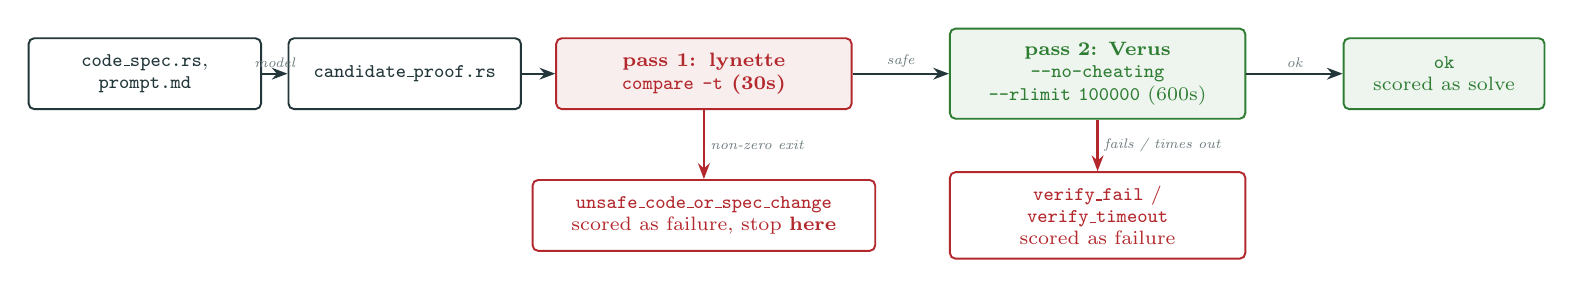
\begin{tikzpicture}[node distance=8mm]
  \node[stage, text width=26mm] (in) at (0,0) {\code{code\_spec.rs},\\\code{prompt.md}};
  \node[stage, text width=26mm] (cand) at (3.3,0) {\code{candidate\_proof.rs}};
  \node[gate,  text width=34mm] (g1) at (7.1,0) {\textbf{pass 1: lynette}\\\code{compare -t}
    (30s)};
  \node[okstage, text width=34mm] (g2) at (12.1,0) {\textbf{pass 2: Verus}\\\code{--no-cheating
    --rlimit 100000} (600s)};
  \node[okstage, text width=22mm] (ok) at (16.5,0) {\code{ok}\\scored as solve};

  \node[stage, draw=lgRed, text=lgRed, text width=40mm] (rej) at (7.1,-1.8)
    {\code{unsafe\_code\_or\_spec\_change}\\scored as failure, stop \textbf{here}};
  \node[stage, draw=lgRed, text=lgRed, text width=34mm] (fail) at (12.1,-1.8)
    {\code{verify\_fail} / \code{verify\_timeout}\\scored as failure};

  \draw[flow]  (in) -- (cand) node[lbl, midway, above] {model};
  \draw[flow]  (cand) -- (g1);
  \draw[flow]  (g1) -- (g2) node[lbl, midway, above] {safe};
  \draw[flow]  (g2) -- (ok) node[lbl, midway, above] {ok};
  \draw[flowr] (g1) -- (rej) node[lbl, midway, right] {non-zero exit};
  \draw[flowr] (g2) -- (fail) node[lbl, midway, right] {fails / times out};
\end{tikzpicture}%
}
\end{center}

\vspace{10pt}
\begin{callout}[lgAccent]
\scriptsize
Only candidates lynette marks \code{safe} ever reach Verus. Everything this deck asks is
about that first pass.
\end{callout}

\end{frame}

% =====================================================================
% Orientation: why is a gate needed at all (motivates Q1 onward, and Q7 later)
\begin{frame}[fragile]{Why a gate is needed at all}

{\scriptsize
ProofGen hands the model one file to edit, and grades it with Verus. But Verus checks a
proof against whatever spec and code that file \emph{contains}, and the model wrote the
whole file.
}

\vspace{5pt}
\begin{defbox}{What Verus checks, vs.\ what the task asks}
\scriptsize
\begin{tabular}{@{}rl@{}}
\textbf{Verus checks:} & $\mathrm{verifies}(S_{\mathrm{cand}}, C_{\mathrm{cand}},
                          P_{\mathrm{cand}}) \in \{0,1\}$: a claim about whatever file the
                          model wrote.\\[4pt]
\textbf{the task asks:} & $\mathrm{solve}(S_{\mathrm{gt}}, C_{\mathrm{gt}})$: a claim about
                          the frozen problem it was actually given.
\end{tabular}\\[6pt]
\scriptsize These coincide only if $S_{\mathrm{cand}}{=}S_{\mathrm{gt}}$ and
$C_{\mathrm{cand}}{=}C_{\mathrm{gt}}$.
\end{defbox}

\vspace{6pt}
\begin{columns}[T]
\begin{column}{0.46\textwidth}
\begin{codebox}[lgTeal]{ground-truth obligation}
\begin{lstlisting}[basicstyle=\ttfamily\scriptsize\color{lgInk}]
ensures
    result == 2 * x,
\end{lstlisting}
\end{codebox}
\end{column}
\begin{column}{0.46\textwidth}
\begin{codebox}[lgRed]{a weakened spec, trivially provable}
\begin{lstlisting}[basicstyle=\ttfamily\scriptsize\color{lgInk}]
ensures
    true,
\end{lstlisting}
\end{codebox}
\end{column}
\end{columns}

\vspace{6pt}
\begin{callout}[lgAccent]
\scriptsize
Absent a filter, a model facing an unprovable obligation could weaken the spec instead of
finding the proof, and Verus would happily verify a different, easier problem it was never
asked to solve. The gate's job is to make ``the spec is still the ground-truth spec, and the
code is still the given code'' true \emph{before} Verus's verdict is treated as an answer to
the actual task.
\end{callout}

\end{frame}

% =====================================================================
% Q1. How many gpt55 ProofGen results are rejected by lynette but accepted by Verus?
\begin{frame}{How this started}

\begin{callout}[lgAccent]
\scriptsize
I was testing ideas against the baseline \textbf{proof-repair} loop. The results would not come
out consistent. That sent me into the ProofGen scoring pipeline, where a filter called
\textbf{lynette} decides whether a candidate reaches Verus at all.
\end{callout}

\vspace{3pt}

\begin{columns}[T]
\begin{column}{0.46\textwidth}
{\scriptsize
\hd{gpt55, ProofGen s0, 946 problems}\\[2pt]
\begin{tabular}{lrrr}
\toprule
 & \textbf{Verus ok} & \textbf{Verus fail} & \textbf{total} \\
\midrule
lynette \good{safe}  & 132 & 118 & 250 \\
lynette \bad{unsafe} & \bad{\textbf{49}} & 647 & 696 \\
\midrule
total & 181 & 765 & 946 \\
\bottomrule
\end{tabular}
}

\vspace{4pt}
{\scriptsize
Pipeline reports \textbf{132 / 946 = 13.95\%}\\
Verus alone accepts \textbf{181 / 946 = 19.13\%}

\vspace{3pt}
\bad{\textbf{The gate is the entire difference: +5.18pp, +37.1\% relative.}}
}
\end{column}

\begin{column}{0.5\textwidth}
{\scriptsize
\hd{Invisible by construction}\\
The harness runs Verus \emph{only} on candidates the gate already passed, so
``gate-rejected but Verus-accepts'' cannot appear in any recorded summary JSON. It became
visible only by re-running Verus on all 946 with the gate bypassed.

\vspace{5pt}
\hd{Not cheating by another route}\\
These 49 verify under \code{--no-cheating}, which rejects \code{assume}, \code{admit}, and
\code{external\_body}. Assume-smuggling is a different cell: 57 of the 118 that pass the gate
and then fail Verus.
}
\end{column}
\end{columns}

\end{frame}

% =====================================================================
% Q2. Take one of those 49: how does the pipeline use lynette, what does it
% see, why does it reject, and why should it have accepted?
\begin{frame}[fragile]{cf148A: how lynette gates a candidate}

\begin{callout}[lgAccent]
\scriptsize
Codeforces \code{cf148A}, gpt55 s0. Smallest of the 14 if-drop cases (47-line
\code{code\_spec.rs}); the model's entire addition is one \code{if}/\code{else}. Its own
gold \code{verified.rs} \good{passes} this same gate, so this is not a problem the gate can
never satisfy: it is wrong about \emph{this candidate}.
\end{callout}

\vspace{3pt}

\begin{center}
\resizebox{0.6\linewidth}{!}{%
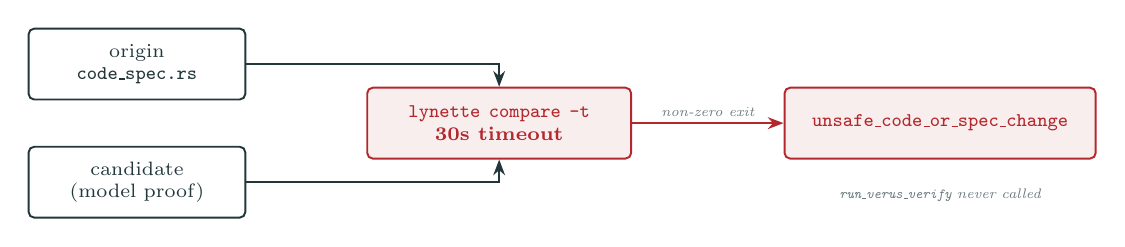
\begin{tikzpicture}[node distance=6mm]
  \node[stage, text width=24mm] (o) at (0,0.75) {origin\\\code{code\_spec.rs}};
  \node[stage, text width=24mm] (c) at (0,-0.75) {candidate\\(model proof)};
  \node[gate,  text width=30mm] (g) at (4.6,0)    {\code{lynette compare -t}\\30s timeout};
  \node[gate,  text width=36mm] (r) at (10.2,0)   {\code{unsafe\_code\_or\_spec\_change}};

  \draw[flow]  (o) -| (g);
  \draw[flow]  (c) -| (g);
  \draw[flowr] (g) -- (r) node[lbl, midway, above] {non-zero exit};
  \node[lbl, below=3mm of r, text width=36mm, align=center] {\code{run\_verus\_verify} never called};
\end{tikzpicture}%
}
\end{center}

\vspace{3pt}
\begin{columns}[T]
\begin{column}{0.4\textwidth}
{\scriptsize
\hd{The call}\\
\code{test\_spec\_code2proof.py:108} calls \code{code\_change\_is\_safe} in target mode:
exactly the gate above. Only candidates marked \code{safe} ever reach
\code{run\_verus\_verify}.

\vspace{4pt}
{\color{lgGrey}\code{count = count + 1;} and \code{i = i + 1;} are byte-identical to the
original.}
}
\end{column}

\begin{column}{0.56\textwidth}
\begin{codebox}[lgGrey]{what the model added: the else branch}
\begin{lstlisting}[basicstyle=\ttfamily\tiny\color{lgInk}]
} else {
    assert(!damaged(i as int, k as int,
        l as int, m as int, n as int));
    assert(count_damaged_spec(k as int,
        l as int, m as int, n as int, i as int)
        == count_damaged_spec(k as int,
        l as int, m as int, n as int, i as int - 1));
}
\end{lstlisting}
\end{codebox}
\end{column}
\end{columns}

\end{frame}

% =====================================================================
\begin{frame}[fragile]{What lynette actually compares}

{\scriptsize Deghosted view of both sides, from \code{lynette compare -t -v}:}

\vspace{3pt}
\begin{columns}[T]
\begin{column}{0.48\textwidth}
\begin{codebox}[lgTeal]{code\_spec.rs, as lynette sees it}
\begin{lstlisting}
while i <= d {
    if i % k == 0 || i % l == 0
        || i % m == 0 || i % n == 0 {
        count = count + 1;
    }
    i = i + 1;
}
\end{lstlisting}
\end{codebox}
\end{column}

\begin{column}{0.48\textwidth}
\begin{codebox}[lgRed]{candidate, as lynette sees it}
\begin{lstlisting}
while i <= d {
    i = i + 1;
}
\end{lstlisting}
\end{codebox}
\end{column}
\end{columns}

\vspace{6pt}
\begin{columns}[T]
\begin{column}{0.48\textwidth}
{\scriptsize
\hd{Why it rejects}\\
\code{deghost.rs:125--147}, the \code{Expr::If} arm: an all-assert \code{else} deghosts to
\code{None}; \code{None.map(...)} is \code{None}; the entire \code{ExprIf} node is dropped,
then-branch included. The counting logic disappears from the candidate's view, and the gate
reports a difference it created itself.
}
\end{column}

\begin{column}{0.48\textwidth}
\begin{callout}[lgGreen]
\scriptsize
\textbf{Why it should have been accepted.} Verus verifies the candidate in 0.4s under
\code{--no-cheating}, and the gold \code{verified.rs} for this problem is \code{safe}. A
complete, correct proof is recorded as tampering because the tool deleted real code before
comparing it.
\end{callout}
\end{column}
\end{columns}

\end{frame}

% =====================================================================
% Q3. How many of the 49 should really be accepted, and what does that do
% to the percentage?
\begin{frame}{44 of the 49 should be accepted}

{\scriptsize gpt55, s0, pin \code{fce8da7}. Each of the 49 re-cut by \emph{cause}:}

\vspace{4pt}
\begin{center}
{\scriptsize
\begin{tabular}{lrl}
\toprule
\textbf{cause} & \textbf{n} & \textbf{call} \\
\midrule
lynette if-drop artifact                         & 20 & \good{\textbf{accept}} \\
subexpression / return-value hoisting            & 11 & \good{\textbf{accept}} \\
inert \code{let old\_x = x;} insertions          & 8  & \good{\textbf{accept}} \\
contract added to a previously-bare helper       & 3  & \good{\textbf{accept}} \\
added \code{use} import only                     & 1  & \good{\textbf{accept}} \\
type annotation only                             & 1  & \good{\textbf{accept}} \\
\code{for} $\to$ \code{while} rewrite            & 3  & \bad{\textbf{reject}} \\
new exec functions added                         & 1  & \bad{\textbf{reject}} \\
genuine semantic edit                            & 1  & \bad{\textbf{reject}} \\
\bottomrule
\end{tabular}
}
\end{center}

\vspace{8pt}
\begin{center}
{\large\bad{\textbf{Corrected: 176 / 946 = 18.60\%} \normalsize(+4.65pp, +33.3\% relative)}}
\end{center}

\end{frame}

% =====================================================================
% Q4. The single-pass effect is modest. Where does the gate actually do damage?
\begin{frame}[fragile]{repair@k oscillates: A $\to$ B $\to$ A}

{\scriptsize
\hd{pass@k drops a rejected sample. repair@k reverts.}\\
A gate rejection does not remove one candidate out of $k$: it resets the trajectory to the
last accepted state and tries again, so the sequence of states bounces \textbf{A} (safe)
$\to$ \textbf{B} (attempt) $\to$ \textbf{A} (reverted), instead of moving forward.
}

\vspace{8pt}
\begin{center}
\begin{codebox}[lgRed]{on rejection: the repair loop's revert}
\begin{lstlisting}
state.current_program = state.last_safe_program
state.last_error      = CODE_SPEC_CHANGED_ERROR
state.solved_round    = max(0, round_index - 1)
\end{lstlisting}
\end{codebox}
\end{center}

\vspace{6pt}
{\scriptsize
\code{current\_program} reverts to the last safe program: what Verus actually receives next
round.\\
\code{last\_error} is set to \code{CODE\_SPEC\_CHANGED\_ERROR}: what the next prompt is told,
whether or not the model actually changed anything.\\
\code{solved\_round} rolls back too, if that reverted program itself verifies.
}

\vspace{6pt}
{\scriptsize\color{lgGrey} One rejection costs pass@k one sample out of $k$. In repair@k it
costs the \emph{chain}: progress is discarded, and the next round starts from the accusation,
not from where the model actually was.}

\end{frame}

% =====================================================================
% Q5. If lynette exists to check that the model didn't tweak spec or code,
% shouldn't the benchmark's own verified.rs always pass against code_spec.rs?
\begin{frame}{Ground truth fails the gate 31.8\% of the time}

{\scriptsize
Every problem ships a \code{verified.rs}: the benchmark's own reference proof, a
known-correct answer to the exact task the model is given. Run the gate against it directly.
}

\vspace{10pt}
\begin{center}
{\scriptsize
\hd{\code{lynette compare -t}\quad\code{code\_spec.rs} vs \code{verified.rs}\quad
($n=946$, pin \code{fce8da7})}\\[6pt]
\begin{tabular}{lrr}
\toprule
 & \textbf{count} & \textbf{share} \\
\midrule
\good{accept}         & 645 & 68.2\% \\
\bad{\textbf{REJECT}} & \bad{\textbf{301}} & \bad{\textbf{31.8\%}} \\
\bottomrule
\end{tabular}
}
\end{center}

\vspace{12pt}
\begin{callout}[lgAccent]
\scriptsize
A third of the benchmark's own correct answers are classified as having tweaked the spec or
the code. The reference proofs are genuine: only one of the 946 fails Verus.
\end{callout}

\end{frame}

% =====================================================================
\begin{frame}[fragile]{cf1200C: the entire objection is a library import}

{\scriptsize The reference proof needs a vstd lemma, so it imports it. Its complete deghosted
difference from \code{code\_spec.rs}:}

\vspace{6pt}
\begin{center}
\begin{codebox}[lgGrey]{cf1200C: verified.rs vs code\_spec.rs, deghosted}
{\ttfamily\scriptsize
\phantom{+ }use vstd::prelude::*;\\
{\color{lgGreen}+ }use vstd::arithmetic::div\_mod::*;
}
\end{codebox}
\end{center}

\vspace{8pt}
{\scriptsize
That is the whole diff, and the gate exits 1. \code{use} items pass through erasure
untouched, so any proof needing a vstd import beyond what \code{code\_spec.rs} already has
can \textbf{never} pass, however clean the proof.
}

\vspace{10pt}
\begin{center}
{\large\bad{\textbf{52 / 52}}}\quad{\scriptsize of \code{verified.rs} files that add a
\code{use} line are rejected. Of the 645 the gate accepts, \textbf{0} add one.}
\end{center}

\end{frame}

% =====================================================================
\begin{frame}[fragile]{lc2094: code\_spec.rs was never fully built}

{\scriptsize The rejection here is not about the proof: \code{code\_spec.rs} is missing
contracts its own reference proof needs, so \code{verified.rs} supplies them and is charged
with tampering for it. Helper \code{count\_digit\_exec}:}

\vspace{4pt}
\begin{center}
{\tiny
\renewcommand{\arraystretch}{0.85}
\begin{tabular}{ll}
\toprule
\textbf{file} & \textbf{what it says about \code{count\_digit\_exec}} \\
\midrule
\code{code.rs}       & bare: \code{fn count\_digit\_exec(...) -> i32 \{} \\
\code{spec.rs}       & absent: states only the target's contract and \code{spec fn}s \\
\code{code\_spec.rs} & an \code{ensures}, but \textbf{no \code{requires}} \\
\code{verified.rs}   & the \code{requires}, plus a second \code{ensures} clause \\
\bottomrule
\end{tabular}
}
\end{center}

\vspace{5pt}
\begin{center}
\begin{codebox}[lgGrey]{the gate's diff: verified.rs filling in what code\_spec.rs left out}
{\ttfamily\tiny\setlength{\baselineskip}{7pt}
\phantom{+ }fn count\_digit\_exec(nums: \&Vec<i32>, digit: i32) -> i32\\[1pt]
{\color{lgGreen}+\ }requires nums.len() <= 100,\\[1pt]
{\color{lgGreen}+\ }\quad forall|i: int| 0<=i<nums.len() ==> 0<=\#[trigger] nums[i]<=9,\\[1pt]
\phantom{+ }ensures c as int == Self::count\_digit(nums@, digit as int, nums.len() as int),\\[1pt]
{\color{lgGreen}+\ }\quad 0 <= c <= nums.len(),
}
\end{codebox}
\end{center}

\end{frame}

% =====================================================================
\begin{frame}{Why this happens, and why nothing caught it}

\begin{columns}[T]
\begin{column}{0.5\textwidth}
{\scriptsize
\hd{Why this happens}\\
\code{code\_spec.rs} is not assembled from \code{code.rs} + \code{spec.rs}. The benchmark's
authoring skill builds it by \emph{back-propagating} from \code{verified.rs} after the proof
succeeds: ``update \code{code\_spec.rs} to match the verified algorithm structure (without
proof, ghost vars, loop invariants, and decreases).'' Contracts are not on that removal list,
which is why \code{code\_spec.rs} carries helper contracts absent from both \code{code.rs}
and \code{spec.rs}. That step is manual, and here it was done incompletely.
}
\end{column}

\begin{column}{0.46\textwidth}
\begin{defbox}{Why nothing caught it}
\scriptsize
The benchmark's consistency checker asserts
\begin{center}
\code{code\_spec.rs} $\subseteq$ \code{verified.rs}
\end{center}
an ordered line-subsequence, one-directional. A contract the author forgot to
back-propagate makes \code{code\_spec.rs} \emph{smaller}, which still satisfies $\subseteq$.
\code{lc2094} passes the benchmark's own QA cleanly.
\end{defbox}
\end{column}
\end{columns}

\vspace{10pt}
\begin{callout}[lgRed]
\scriptsize
The model is handed an under-specified file, and the frozen ``ground truth'' it is measured
against is a partially back-propagated proof artifact, not the stated specification in
\code{spec.rs}.
\end{callout}

\end{frame}

% =====================================================================
% Q6. Summary -- every category where lynette rejects a proof that should pass
\begin{frame}[fragile]{Five ways the gate manufactures tampering (1/2)}

\begin{callout}[lgAccent]
\scriptsize
The gate tests \textbf{equality} of the proof-erased remainder. ProofGen needs
\textbf{extension}: output = original + proof-only additions. Equality cannot express
``additions are allowed,'' and the erasure itself is buggy. Every category below follows
from that.
\end{callout}

\vspace{8pt}
\begin{columns}[T]
\begin{column}{0.48\textwidth}

\begin{codebox}[lgGrey]{1. a ghost-only \code{else} deletes the whole \code{if}}
{\ttfamily\scriptsize
\phantom{+ }if a[i] > t \{\\
\phantom{+ }\quad cnt = cnt + 1;\\
{\color{lgGreen}+\ }\} else \{\\
{\color{lgGreen}+\ }\quad proof \{ assert(cnt as int\\
{\color{lgGreen}+\ }\qquad == count\_prefix(a@, i+1)); \}\\
\phantom{+ }\}
}
\end{codebox}

\vspace{5pt}
{\scriptsize\color{lgGrey}Lynette then sees nothing: the whole statement, \code{cnt = cnt +
1} included, is gone. A comment-only \code{else} does it too.}

\end{column}
\begin{column}{0.48\textwidth}

\begin{codebox}[lgGrey]{2. an added \code{use} import}
{\ttfamily\scriptsize
{\color{lgGreen}+\ }use vstd::arithmetic::div\_mod::*;
}
\end{codebox}

\vspace{5pt}
{\scriptsize\color{lgGrey}\code{use} items pass through erasure untouched
(\code{cf1200C}, Q5).}

\vspace{14pt}
\begin{codebox}[lgGrey]{4. a ghost witness written \code{let}, not \code{let ghost}}
{\ttfamily\scriptsize
{\color{lgGreen}+\ }let old\_best = best;\\
\phantom{+\ }\quad // read only inside asserts
}
\end{codebox}

\end{column}
\end{columns}

\end{frame}

% =====================================================================
\begin{frame}[fragile]{Five ways the gate manufactures tampering (2/2)}

\vspace{18pt}
\begin{columns}[T]
\begin{column}{0.48\textwidth}

\begin{codebox}[lgGrey]{3. \code{invariant}/\code{decreases} on a bare \code{loop}}
{\ttfamily\scriptsize
\phantom{+ }loop\\
{\color{lgGreen}+\ }\quad invariant i <= n,\\
{\color{lgGreen}+\ }\quad decreases n - i,\\
\phantom{+ }\{
}
\end{codebox}

\vspace{6pt}
{\scriptsize\color{lgGrey}Verus cannot verify a bare loop without them: no correct proof of
such a problem can pass.}

\end{column}
\begin{column}{0.48\textwidth}

\begin{codebox}[lgGrey]{5. a contract on a helper that shipped bare}
{\ttfamily\scriptsize
{\color{lgRed}-\ }fn helper(v: \&Vec<i32>) -> usize \{\\
{\color{lgGreen}+\ }fn helper(v: \&Vec<i32>) -> usize\\
{\color{lgGreen}+\ }\quad ensures result <= v.len(),\\
{\color{lgGreen}+\ }\{
}
\end{codebox}

\vspace{6pt}
{\scriptsize\color{lgGrey}Without it, the caller cannot be proven at all.}

\end{column}
\end{columns}

\end{frame}

% =====================================================================
% Q7. Why does this happen? What behaviour do we want, versus what lynette
% was built for?
\begin{frame}{The relation we need, and the one we have}

{\scriptsize
The gate's job is \textbf{task identity}: is the candidate still an answer to the problem
that was handed out?
}

\vspace{8pt}
\begin{defbox}{Want vs.\ have}
\scriptsize
\begin{tabular}{@{}rl@{}}
\textbf{want:} & $\mathrm{accept}(O,F) \iff F = O+\Delta,\ \text{every } \delta\in\Delta$
                 \text{ proof-only} \quad\textit{(extension)}\\[4pt]
\textbf{have:} & $\mathrm{accept}(O,F) \iff \mathrm{erase}(O) = \mathrm{erase}(F)$
                 \quad\textit{(equality)}\\
\end{tabular}
\end{defbox}

\vspace{10pt}
{\scriptsize
Equality is an \textbf{equivalence relation}: symmetric. Extension is a \textbf{partial
order}: antisymmetric. ``Additions are allowed, in one direction only'' is not expressible
in a symmetric relation. That is the entire defect, stated once. Every category in Q6 is an
addition that an equality test structurally cannot represent.
}

\end{frame}

% =====================================================================
\begin{frame}{Why lynette is built that way}

{\scriptsize
lynette is AutoVerus's tool, and \code{compare} is literally the precondition its
\textbf{merge} asserts (\code{fmerge\_files}). To splice proof content from one candidate
into another you must know they are the \emph{same program modulo proof}: for merging,
equality is exactly the right relation. VeriContest imported that check through
\code{evaluation.util.code\_change\_is\_safe} and repurposed it as a cheating detector.
}

\vspace{8pt}
\begin{center}
\resizebox{0.95\linewidth}{!}{%
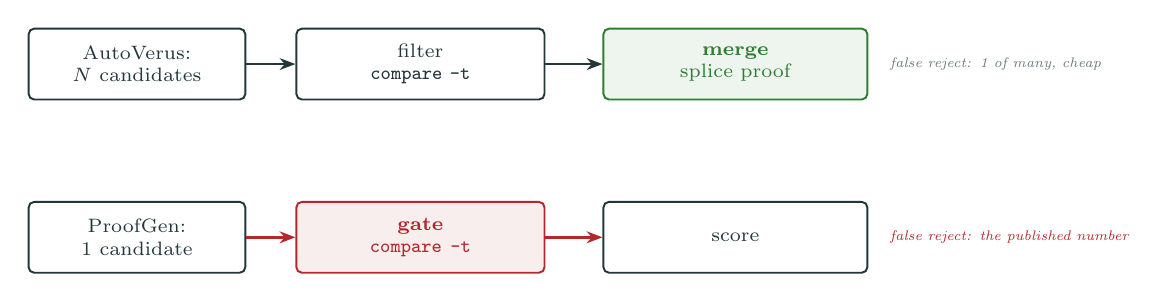
\begin{tikzpicture}[node distance=6mm]
  \node[stage,   text width=24mm] (a1) at (0,1.1)   {AutoVerus:\\$N$ candidates};
  \node[stage,   text width=28mm] (a2) at (3.6,1.1) {filter\\\code{compare -t}};
  \node[okstage, text width=30mm] (a3) at (7.6,1.1) {\textbf{merge}\\splice proof};
  \node[lbl, right=2mm of a3, text width=32mm] {false reject: 1 of many, cheap};

  \node[stage, text width=24mm] (b1) at (0,-1.1)   {ProofGen:\\1 candidate};
  \node[gate,  text width=28mm] (b2) at (3.6,-1.1) {gate\\\code{compare -t}};
  \node[stage, text width=30mm] (b3) at (7.6,-1.1) {score};
  \node[lbl, right=2mm of b3, text width=32mm, text=lgRed] {false reject: the published number};

  \draw[flow]  (a1) -- (a2); \draw[flow]  (a2) -- (a3);
  \draw[flowr] (b1) -- (b2); \draw[flowr] (b2) -- (b3);
\end{tikzpicture}%
}
\end{center}

\vspace{8pt}
\begin{callout}[lgAccent]
\scriptsize
\textbf{The cost asymmetry flips on import.} AutoVerus filters $N$ candidates: a false reject
is a rational trade. ProofGen scores one candidate per problem: the same false reject is
measurement error in a published number. Same behaviour, opposite economics. The tool is not
malfunctioning: it is being used outside its design contract.
\end{callout}

\end{frame}

% =====================================================================
\begin{frame}{The benchmark already knows the right relation}

{\scriptsize VeriContest's own authoring checker asserts:}

\vspace{6pt}
\begin{center}
\begin{defbox}{extension, already, in the QA}
\scriptsize
\code{code\_spec.rs} $\subseteq$ \code{verified.rs} \quad(ordered subsequence, i.e.\
extension)
\end{defbox}
\end{center}

\vspace{8pt}
\begin{center}
{\scriptsize
\begin{tabular}{lr}
\toprule
\textbf{check} & \textbf{pass rate} \\
\midrule
authoring checker ($\subseteq$, extension) & \good{\textbf{946 / 946}} \\
scoring pipeline (\code{compare -t}, equality) & \bad{\textbf{645 / 946}} \\
\bottomrule
\end{tabular}
}
\end{center}

\vspace{12pt}
\begin{callout}[lgAccent]
\scriptsize
\textbf{The benchmark defines the task as extension in its QA, and scores it as equality in
its pipeline.}
\end{callout}

\end{frame}

% =====================================================================
% Q8. So what do we do?
\begin{frame}{So what do we do? Three paths}

\begin{columns}[T]
\begin{column}{0.46\textwidth}
{\scriptsize
\hd{1. Drop the gate.}\\
Trust the model not to touch spec or code, and spend the effort on repair@k instead.

\vspace{7pt}
\hd{2. Build our own AST-based gate.}\\
\code{vgate}, in \code{tools/vgate/}, with minimal engineering. It also identifies where
\code{code\_spec.rs} needs patching against \code{verified.rs}.

\vspace{7pt}
\hd{3. Treat the filter as a general problem.}\\
Given a spec $S$, code $C$, and an arbitrary file $Z$, decide by AST whether $Z$ has the same
spec as $S$ and the same code as $C$.
}
\end{column}

\begin{column}{0.5\textwidth}
{\scriptsize\hd{Where each lands}}\\[3pt]
{\scriptsize
\begin{tabular}{lrr}
\toprule
\textbf{gate} & \textbf{GT accepted} & \textbf{gpt55 pass@1} \\
\midrule
\code{lynette compare -t} (current) & 68.2\% & 13.95\% \\
\code{vgate} (prototype)   & \good{\textbf{83.4\%}} & \good{\textbf{15.12\%}} \\
no gate at all                      & 99.9\% & 19.13\% \\
\bottomrule
\end{tabular}
}

\vspace{10pt}
\begin{callout}[lgGrey]
\tiny
\code{vgate} is a prototype: validated on the 946 reference proofs and on gpt55 s0 only,
never replayed against the recorded candidate runs, with an unresolved \code{let} vs
\code{let ghost} policy and four known gaps in its README.
\end{callout}
\end{column}
\end{columns}

\end{frame}

\end{document}
